% !TeX root = ../main.tex
% -*- coding: utf-8 -*-

\chapter{绪论}
\label{1}


\section{研究背景与意义}

近年来,科技迅速发展,计算资源日益丰富,计算能力得到显著提升,我们正在进入人工智能(Artificial Intelligence, AI)\cite{winston1984artificial}的时代。随着互联网的的快速发展,产生了海量的数据,得益于深度神经网络(Deep Neural Network, DNN)\cite{sze2017efficient}强大的数据处理能力,DNN已经成为应用最广泛的人工智能方法之一。自DNN在计算机视觉\cite{he2016identity,cortes2015advances,simonyan2014very},语音识别\cite{nassif2019speech},自然语言处理\cite{collobert2011natural,wu2016google,xiong2016achieving}等方面上突破性应用以来,使用DNN的应用数量呈爆炸式增长。这些DNN应用被应用到从自动驾驶\cite{chen2015deepdriving}到癌症检测\cite{esteva2017dermatologist}到玩复杂的游戏\cite{silver2017mastering}等无数应用中。并且在许多这些领域中,DNN已经能够超越人类的准确性。

DNN在许多领域取得巨大成功,为人类社会生活带来极大便利的同时,也带来了非常严重的侵犯知识产权(Intellectual Property, IP)问题。训练一个大型的高性能的DNN模型都离不开该领域专家的专业知识、规模巨大的数据集以及大量的训练时间和强大的计算资源,具体体现在以下三个方面:

\begin{enumerate}
	\renewcommand{\labelenumi}{\theenumi)}
	\item 人力资源,对于不同场景不同目的的DNN模型,需要不同领域的知识,包含对模型结构的设计分析、模型参数的调试校验等;
	\item 大量的训练数据,模型所有者要在特定领域训练出一个高性能的模型,通常需要该领域大量的数据,并且需要覆盖到应用场景中的各种情况,这些数据的获取和整理本身就需要昂贵的价格,有的领域的数据还涉及到隐私性问题;
	\item 昂贵的计算资源和大量的训练时间,DNN模型的规模越来越大,层数越来越多,需要的训练时间也越多,并且训练过程中也需要越来越多的计算资源支持,才能对网络权重等进行精确的调整,这些都是巨额的经济成本。如GPT-3\cite{brown2020language},包含了1750亿参数,仅训练成本需花费460万美元以上。
\end{enumerate}

所以高性能DNN模型是模型所有者智慧的结晶,同时需要高额的经济开销,模型所有者享有DNN模型的知识产权\cite{chen2018performance,darvish2019deepsigns}。

模型所有者出于学术目的将DNN模型放到开源社区上。或者,使用机器学习即服务(Machine Learning as a Service, MLaaS)\cite{ribeiro2015mlaas}的商业模式,即MLaaS平台通过训练好的DNN模型来向用户提供应用程序接口(Application Programming Interface, API)\cite{ofoeda2019application},用户可以通过支付一定的费用来使用API。或者,训练好的DNN模型将成为像我们日常商品一样的消费品,它们由不同的公司或个人进行训练,由不同的供应商分发,最终由用户消费。如图\ref{DNN模型服务和盗窃示意图}所示,这样的方式极大的方便了科研工作者和一般的消费者,但是不法分子却可以以比模型所有者低很多的成本复制一个替代模型,用于自己盈利。

\begin{figure}[htbp]%%图,[htbp]是浮动格式
	\centering
	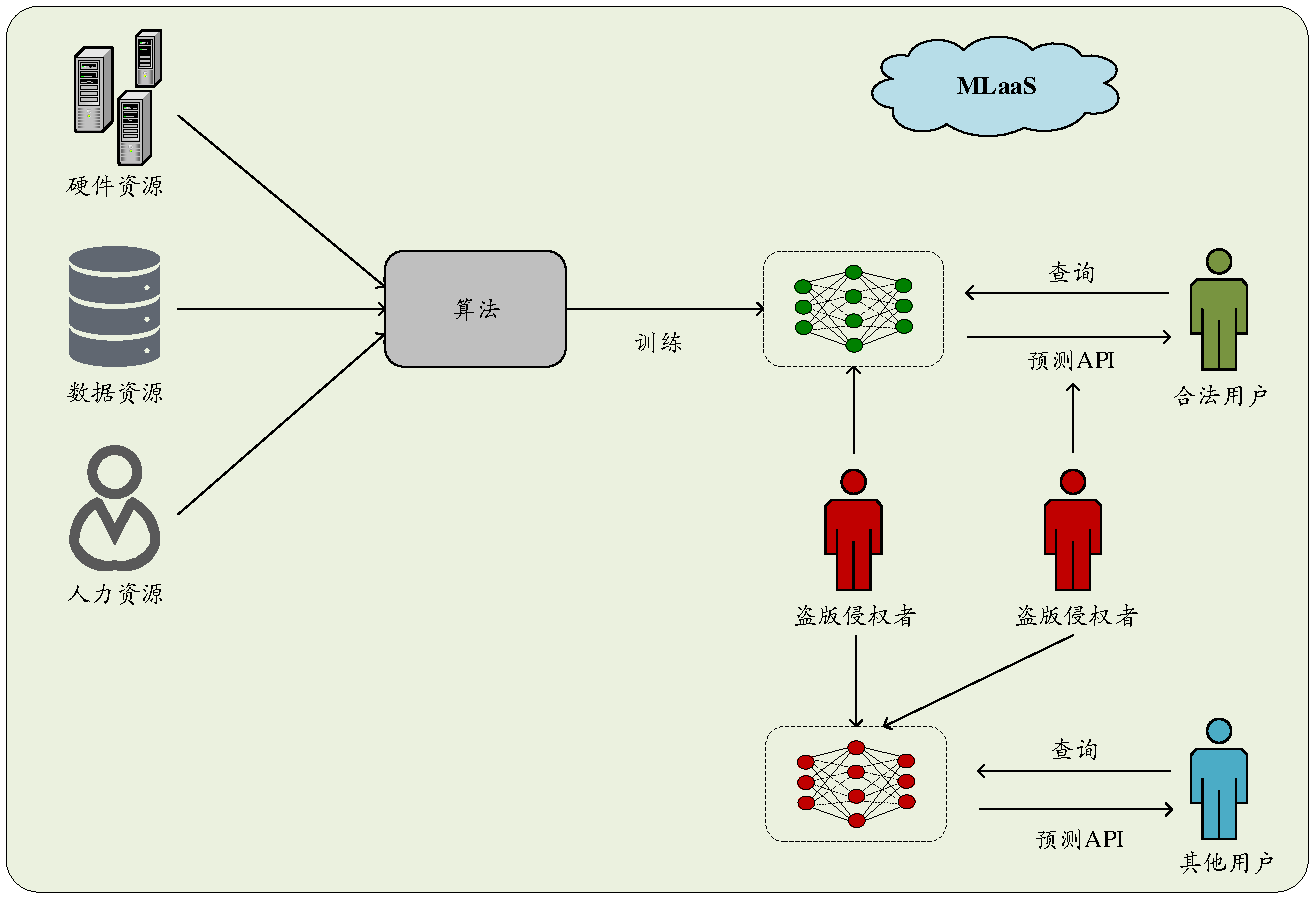
\includegraphics[width=14.5cm,height=9cm]{DNN模型服务和盗窃示意图.pdf}
	%	\centerline{原始样本}
	\setlength{\abovecaptionskip}{5mm} %图片标题与图片距离
	\caption{DNN模型服务和盗窃示意图}
	\label{DNN模型服务和盗窃示意图}
	\end {figure}
	
所以如何在训练和部署时保护DNN模型所有者的知识产权是AI领域亟待解决的问题。


\section{相关研究现状}

作为一种数字产品,DNN模型不仅凝结了设计者的智慧,还需要消耗大量的训练数据和昂贵的计算资源。近年来,拥有先进的的模型带来的工业优势已经被人们广泛认可,这开始激发一些不法分子窃取这些模型的攻击\cite{tramer2016stealing,duddu2018stealing}。现在可以明确的是,DNN模型将在未来的IT发展中发挥核心作用,因此保护这些模型的必要性显得更加突出。1994年,Van Schyndel等人\cite{van1994digital}第一次提出数字水印的概念,将标记隐蔽的嵌入到如音频、视频等数字内容中,来识别其所有权,具体来说,版权所有者通过显示此类标记的存在可以证明其对内容的所有权。DNN模型也是一种数字产品,所以,许多研究者从数字媒体水印得到启发,从而设计模型水印和模型指纹用于解决DNN模型的所有权问题。

模型水印是解决DNN模型知识产权问题的主要方式之一,Uchida等人\cite{uchida2017embedding}在2017年首次提出了在DNN模型中嵌入水印的通用框架。该方法是一种白盒的模式,通过训练时使用正则化器,并且这种正则化在参数中引入了所需要的统计偏差来作为嵌入的水印。模型所有者清楚模型内部的细节,并且可以提取嵌入的水印,以此来作为模型所有权的依据\cite{nagai2018digital}。Fan等人\cite{fan2019rethinking}提出了一种在DNN模型中嵌入数字护照的方案,嵌入数字护照的要点是设计和训练DNN模型,使得在伪造护照的情况下DNN的推断性能显著下降,而真正的护照可以通过查找预定签名来验证。Chen等人\cite{chen2018deepmarks}提出了一种新颖的端到端框架,该框架同时依赖于用户和模型,它需要为每一个用户分配一个代码向量,并将该信息嵌入到可训练权重的的概率密度函数中,同时保持模型的准确性。不同于白盒的模式,另一种黑盒的模式,可以在不访问模型内部的情况下,通过特定的输入输出来验证模型的所有权。Le等人\cite{le2020adversarial}提出了一种零比特水印算法,该算法标记模型的操作本身,稍微调整它的决策边界,来使特定的查询得到特定的输出。在减少模型性能损失的同时,该算法可以远程操作DNN或API服务,通过少量的查询提取水印。Zhang等人\cite{zhang2018protecting}提出了一种水印植入方法,将水印注入DNN模型。通过扩展DNN的内在泛化和记忆能力,使得模型能够在训练时学习特意制作的水印,然后在推断时激活预先指定的预测。Adi等人\cite{adi2018turning}提出了利用模型的后门机制当作DNN模型水印。后门通常是DNN将输入预测为错误的标签,虽然在大多数情况下这是不可取的,但是却可以将为DNN模型制作水印的任务转化为设计后门的任务。这些黑盒的方法利用对抗性样本作为触发集,或者使用一组特定的训练样本,然后根据特殊样本的输出来提取水印。因此黑盒的方法在所有权验证中不需要访问模型的权重参数。Rouhani等人\cite{rouhani2018deepsigns}提出了一种端到端的IP保护框架DeepSigns,可以在DNN模型中插入连贯的数字水印。DeepSigns引入了一种通用水印方法,不同于直接将水印信息嵌入到模型的权重中,DeepSigns将任意N位字符串嵌入到各层激活集的概率密度函数中,这意味着水印信息嵌入在DNN的动态内容中,并且只能通过特定的输入数据来触发,并且对权重矩阵等静态属性没有影响。但是DNN模型水印的嵌入步骤总是会对原始进行修改。具体来说,白盒水印修改模型内部,比如模型权重,激活函数等,而黑盒水印通过特殊的训练调整模型来指定特定的输出。这些修改将会影响DNN模型在原始任务上的性能。

模型指纹是解决DNN模型知识产权问题的又一主流方法。不同与模型水印,模型指纹不需要对模型本身进行修改,而是利用模型本身来寻找和提取一些独特的特征作为模型指纹,一般来说,模型指纹不会影响模型的性能。Zhao等人\cite{zhao2020afa}提出了一种新的DNN模型指纹技术,该技术旨在提取模型本身的固有特征,而不是嵌入额外的水印。具体来说,该方法选择一组专门设计的对抗性样本作为模型指纹特征,称为对抗性标记,相比于其他不相关的模型,它可以更好的转移到从原始模型派生出的模型上。与Zhao等人\cite{zhao2020afa}的方法类似,Lukas等人\cite{lukas2019deep}提出了一种用于DNN分类器的指纹识别方法,该方法从源模型中提取一组输入,以便只有源模型的派生模型在此类输入的分类上与源模型一致。这些输入是可转移对抗性样本的一个子类,它们的目标标签会从源模型转移到其派生模型上。Cao等人\cite{cao2021ipguard}针对DNN分类器提出了一种名叫IPGuard的指纹方法,该方法的关键是DNN分类器可以由其分类边界唯一的表示。基于这一原理,IPGuard在模型所有者的DNN分类器分类边界上提取了一些数据点,并使用它们对分类器进行指纹识别,如果DNN分类器对大多数指纹数据点预测相同的标签,那么该模型被认为是模型所有者分类器的盗版。Li等人\cite{li2021novel}提出了一种适用于生成对抗网络(Generative Adversarial Network, GAN)\cite{goodfellow2020generative}知识产权保护的指纹识别方案。该方案从目标GAN和分类器构建了一个复合深度学习模型,然后从该复合模型中生成隐蔽的指纹样本,并将其注册到分类器中进行有效的所有权验证。Dong等人\cite{dong2021fingerprinting}针对DNN水印和指纹容易受到最抗性训练攻击,不适用于多出口DNN模型的IP验证的问题,提出了一种根据推理时间而不是推理预测的结果来为多出口模型建立指纹的新方法。

模型窃取攻击涉及到模型的修改,主要包括模型微调,模型剪枝,模型压缩等。模型微调通常用于迁移学习,可以重新调整模型以更改模型参数,同时保持模型的性能。通过微调现有的模型,可以派生出许多功能相似的模型。模型剪枝是是部署DNN模型的常见方法,通过参数修剪来减少DNN的内存和计算开销,而盗窃者可能会使用修剪来删除水印或指纹。模型压缩中常见的是知识蒸馏,通过将大模型中的知识蒸馏到小模型中,可以显著降低模型的训练成本,内存需求和计算开销,同时达到与大模型接近的性能。研究\cite{hinton2015distilling}表明甚至不需要原始训练数据就可以直接利用API蒸馏模型,因此蒸馏常被用来派生模型。

虽然模型水印和模型指纹在保护模型知识产权方面已经取得了很大的进展,但是无论是水印还是指纹都容易受到歧义攻击\cite{fan2019rethinking,li2019piracy},歧义攻击是指通过为DNN模型伪造其他水印或指纹来对所有权验证产生干扰。直觉上,如果模型盗窃者可以在水印模型上嵌入第二个水印或者提取第二个指纹,那么该模型的知识产权归属存在巨大的歧义。

\section{本文主要工作}

为了解决DNN模型的知识产权问题,本文提出了近边界数据,一种分布在分类边界附近的特殊样本。模型指纹\cite{cao2021ipguard}使用对抗性样本抽象地反映模型分类边界,同一组对抗性样本的输入,其引起的决策模式的变化可以用于比较模型知识的相似性,但这种方法是脆弱的,对模型的任意操作都有可能破坏这种特性。因此,我们不直接比较决策模式的变化,它是不可信任的,而是比较对抗性样本与决策边界的距离。有意思的是大多数对抗性样本都是位于决策边界附近的,也就是说,它们与决策边界的距离很近。对抗性样本的这种性质被我们所利用并构造近边界数据,经过测试我们发现绝大多数的模型窃取方法都无法改变这种结果,即使样本分类被影响,其仍然位于分类边界附近。近边界数据背后的意义是如果被用于所有权验证如果两个模型的决策模式相似,参与训练的近边界数据一定可以反映出来。受这个特性的启发,将近边界数据作为水印验证所有权是传统的思路,即使不会对模型的精度造成影响,这样的水印也是脆弱的,很难抵御歧义攻击,因此我们提出由近边界数据驱动的所有权推断方法,其思想是构造私有的近边界数据,当验证一个模型的所有权时,模型所有者和盗窃者分别提供各自的私有近边界数据,距离分类边界最近的被推断获得所有权。

本文的主要贡献如下:

\begin{enumerate}
	\renewcommand{\labelenumi}{\theenumi)}
	\item 揭示了当前所有权验证方案的脆弱性并确认了数据驱动推断所有权的有效性。
	\item 提出了利用对抗性样本构造近边界数据以抵御模型窃取攻击。
	\item 设计了基于DCGAN 的近边界数据生成器,并通过该生成器构造了私有化的近边界数据,提出了一种损失函数用以微调源模型的目标分类边界,增加推断所有权的置信度。
	\item 在ResNet18 上进行了广泛的实验,实验结果证明了近边界数据在推断模型所有权上的显著效果。
\end{enumerate}

\section{本文组织架构}

本文对模型的近边界数据进行了研究,并提出了生成私有近边界数据的方法以及一种基于近边界数据的模型所有权推断方法。全文共分为六个章节,每个章节的主要内容如下:

第一章:绪论。本章首先介绍了DNN模型在当今时代的广泛应用和训练的昂贵成本,引出了保护DNN模型知识产权的必要性和重大意义,然后介绍了模型水印和模型指纹两种保护方法的研究现状,并针对相关研究存在的问题提出了本文的研究内容,最后简要说明了各个章节的内容安排。

第二章:技术背景。本章主要介绍了深度神经网络的结构和相关概念,对抗性攻击和生成对抗网络的原理,常见的模型窃取攻击方式和模型知识产权保护方法。

第三章:基于生成对抗网络特征提取的近边界数据研究。本章首先给出了近边界数据的概念,然后详细介绍了选择CW算法生成对抗性样本的原因,最后给出了本文基于生成对抗网络生成私有化近边界数据的流程和微调源模型的设计。

第四章:基于近边界数据的模型所有权推断方法研究。本章首先阐述了所有权验证和数据集推断的局限性,然后提出了本文方法的设计目标,并详细说明了本文的方法流程,最后利用假设检验来比对结果。

第五章:基于近边界数据的模型所有权推断方法分析。本章在resnet18的基础上,对数据的近边界性,微调模型分类边界的影响,近边界推断模型所有权的有效性以及近边界数量的伸缩性做了详细的实验,证明了本文提出方法在推断模型所有权时的有效性。

第六章:总结与展望。本章总结了本文提出的方法,并针对可能的改进提出了未来工作的展望。
